\begin{auf}
    851
\end{auf}
Weißes Licht fällt aus der Luft kommend senkrecht auf eine Ölschicht (Dicke $d=0.7mm$; Brechzahl $n_2=1.5$), die sich auf einer Wasseroberfläche (Brechzahl $n_3=1.33$) ausgebreitet hat.
\begin{enumerate}
    \item[a] Wie groß ist der Gangunterschied zweier interferierender Wellen und an welcher	Grenzfläche tritt ein Phasensprung auf?
    \item[b] Wie lauten die Interferenzbedingungen für sich maximal verstärkende und sich gegenseitig auslöschende Lichtwellen?
    \item[c] Welche Wellenlängen werden im sichtbaren Bereich ($\lambda=380_{\cdots}780nm$) ausgelöscht?
\end{enumerate}
\begin{figure}[h]
    \centering
    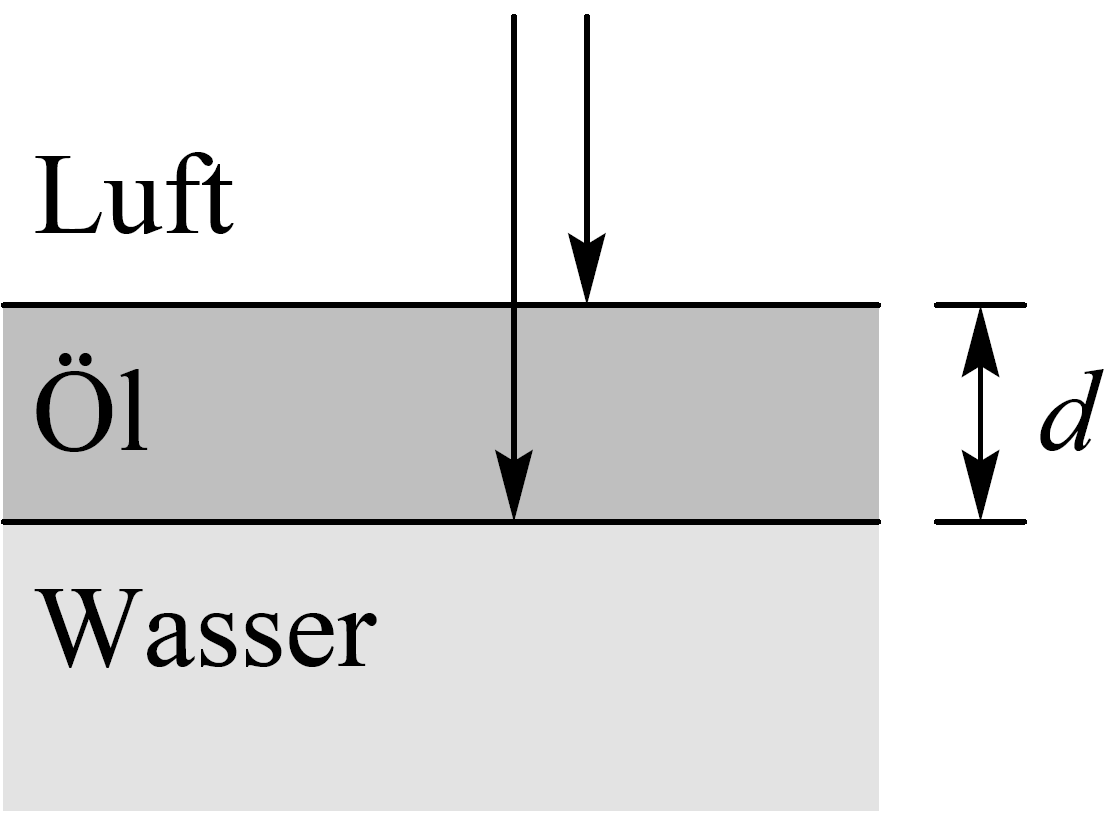
\includegraphics[height=5cm]{images/851_0.png}
    \caption{Versuchsaufbau Aufgabe 851}
\end{figure}